\documentclass[twoside]{book}

% Packages required by doxygen
\usepackage{fixltx2e}
\usepackage{calc}
\usepackage{doxygen}
\usepackage[export]{adjustbox} % also loads graphicx
\usepackage{graphicx}
\usepackage[utf8]{inputenc}
\usepackage{makeidx}
\usepackage{multicol}
\usepackage{multirow}
\PassOptionsToPackage{warn}{textcomp}
\usepackage{textcomp}
\usepackage[nointegrals]{wasysym}
\usepackage[table]{xcolor}

% Font selection
\usepackage[T1]{fontenc}
\usepackage[scaled=.90]{helvet}
\usepackage{courier}
\usepackage{amssymb}
\usepackage{sectsty}
\renewcommand{\familydefault}{\sfdefault}
\allsectionsfont{%
  \fontseries{bc}\selectfont%
  \color{darkgray}%
}
\renewcommand{\DoxyLabelFont}{%
  \fontseries{bc}\selectfont%
  \color{darkgray}%
}
\newcommand{\+}{\discretionary{\mbox{\scriptsize$\hookleftarrow$}}{}{}}

% Page & text layout
\usepackage{geometry}
\geometry{%
  a4paper,%
  top=2.5cm,%
  bottom=2.5cm,%
  left=2.5cm,%
  right=2.5cm%
}
\tolerance=750
\hfuzz=15pt
\hbadness=750
\setlength{\emergencystretch}{15pt}
\setlength{\parindent}{0cm}
\setlength{\parskip}{3ex plus 2ex minus 2ex}
\makeatletter
\renewcommand{\paragraph}{%
  \@startsection{paragraph}{4}{0ex}{-1.0ex}{1.0ex}{%
    \normalfont\normalsize\bfseries\SS@parafont%
  }%
}
\renewcommand{\subparagraph}{%
  \@startsection{subparagraph}{5}{0ex}{-1.0ex}{1.0ex}{%
    \normalfont\normalsize\bfseries\SS@subparafont%
  }%
}
\makeatother

% Headers & footers
\usepackage{fancyhdr}
\pagestyle{fancyplain}
\fancyhead[LE]{\fancyplain{}{\bfseries\thepage}}
\fancyhead[CE]{\fancyplain{}{}}
\fancyhead[RE]{\fancyplain{}{\bfseries\leftmark}}
\fancyhead[LO]{\fancyplain{}{\bfseries\rightmark}}
\fancyhead[CO]{\fancyplain{}{}}
\fancyhead[RO]{\fancyplain{}{\bfseries\thepage}}
\fancyfoot[LE]{\fancyplain{}{}}
\fancyfoot[CE]{\fancyplain{}{}}
\fancyfoot[RE]{\fancyplain{}{\bfseries\scriptsize Generated by Doxygen }}
\fancyfoot[LO]{\fancyplain{}{\bfseries\scriptsize Generated by Doxygen }}
\fancyfoot[CO]{\fancyplain{}{}}
\fancyfoot[RO]{\fancyplain{}{}}
\renewcommand{\footrulewidth}{0.4pt}
\renewcommand{\chaptermark}[1]{%
  \markboth{#1}{}%
}
\renewcommand{\sectionmark}[1]{%
  \markright{\thesection\ #1}%
}

% Indices & bibliography
\usepackage{natbib}
\usepackage[titles]{tocloft}
\setcounter{tocdepth}{3}
\setcounter{secnumdepth}{5}
\makeindex

% Hyperlinks (required, but should be loaded last)
\usepackage{ifpdf}
\ifpdf
  \usepackage[pdftex,pagebackref=true]{hyperref}
\else
  \usepackage[ps2pdf,pagebackref=true]{hyperref}
\fi
\hypersetup{%
  colorlinks=true,%
  linkcolor=blue,%
  citecolor=blue,%
  unicode%
}

% Custom commands
\newcommand{\clearemptydoublepage}{%
  \newpage{\pagestyle{empty}\cleardoublepage}%
}

\usepackage{caption}
\captionsetup{labelsep=space,justification=centering,font={bf},singlelinecheck=off,skip=4pt,position=top}

%===== C O N T E N T S =====

\begin{document}

% Titlepage & ToC
\hypersetup{pageanchor=false,
             bookmarksnumbered=true,
             pdfencoding=unicode
            }
\pagenumbering{roman}
\begin{titlepage}
\vspace*{7cm}
\begin{center}%
{\Large Exp\+\_\+\+Lab\+\_\+\+Assignment\+\_\+3 }\\
\vspace*{1cm}
{\large Generated by Doxygen 1.8.11}\\
\end{center}
\end{titlepage}
\clearemptydoublepage
\tableofcontents
\clearemptydoublepage
\pagenumbering{arabic}
\hypersetup{pageanchor=true}

%--- Begin generated contents ---
\chapter{Hierarchical Index}
\section{Class Hierarchy}
This inheritance list is sorted roughly, but not completely, alphabetically\+:\begin{DoxyCompactList}
\item \contentsline{section}{camera\+\_\+manager.\+camera\+\_\+manager\+\_\+fnct}{\pageref{classcamera__manager_1_1camera__manager__fnct}}{}
\item State\begin{DoxyCompactList}
\item \contentsline{section}{state\+\_\+manager.\+F\+\_\+\+Track}{\pageref{classstate__manager_1_1F__Track}}{}
\item \contentsline{section}{state\+\_\+manager.\+M\+I\+R\+O\+\_\+\+Find}{\pageref{classstate__manager_1_1MIRO__Find}}{}
\item \contentsline{section}{state\+\_\+manager.\+M\+I\+R\+O\+\_\+\+Normal}{\pageref{classstate__manager_1_1MIRO__Normal}}{}
\item \contentsline{section}{state\+\_\+manager.\+M\+I\+R\+O\+\_\+\+Play}{\pageref{classstate__manager_1_1MIRO__Play}}{}
\item \contentsline{section}{state\+\_\+manager.\+M\+I\+R\+O\+\_\+\+Sleep}{\pageref{classstate__manager_1_1MIRO__Sleep}}{}
\item \contentsline{section}{state\+\_\+manager.\+N\+\_\+\+Track}{\pageref{classstate__manager_1_1N__Track}}{}
\end{DoxyCompactList}
\end{DoxyCompactList}

\chapter{Class Index}
\section{Class List}
Here are the classes, structs, unions and interfaces with brief descriptions\+:\begin{DoxyCompactList}
\item\contentsline{section}{\hyperlink{classcamera__manager_1_1camera__manager__fnct}{camera\+\_\+manager.\+camera\+\_\+manager\+\_\+fnct} \\*Class to manage the camera }{\pageref{classcamera__manager_1_1camera__manager__fnct}}{}
\item\contentsline{section}{\hyperlink{classstate__manager_1_1F__Track}{state\+\_\+manager.\+F\+\_\+\+Track} \\*Find track state of the smach machine }{\pageref{classstate__manager_1_1F__Track}}{}
\item\contentsline{section}{\hyperlink{classstate__manager_1_1MIRO__Find}{state\+\_\+manager.\+M\+I\+R\+O\+\_\+\+Find} \\*Find state of the smach machine }{\pageref{classstate__manager_1_1MIRO__Find}}{}
\item\contentsline{section}{\hyperlink{classstate__manager_1_1MIRO__Normal}{state\+\_\+manager.\+M\+I\+R\+O\+\_\+\+Normal} \\*Normal state of the smach machine }{\pageref{classstate__manager_1_1MIRO__Normal}}{}
\item\contentsline{section}{\hyperlink{classstate__manager_1_1MIRO__Play}{state\+\_\+manager.\+M\+I\+R\+O\+\_\+\+Play} \\*Play state of the smach machine }{\pageref{classstate__manager_1_1MIRO__Play}}{}
\item\contentsline{section}{\hyperlink{classstate__manager_1_1MIRO__Sleep}{state\+\_\+manager.\+M\+I\+R\+O\+\_\+\+Sleep} \\*Sleep state of the smach machine }{\pageref{classstate__manager_1_1MIRO__Sleep}}{}
\item\contentsline{section}{\hyperlink{classstate__manager_1_1N__Track}{state\+\_\+manager.\+N\+\_\+\+Track} \\*Normal track state of the smach machine }{\pageref{classstate__manager_1_1N__Track}}{}
\end{DoxyCompactList}

\chapter{File Index}
\section{File List}
Here is a list of all documented files with brief descriptions\+:\begin{DoxyCompactList}
\item\contentsline{section}{scripts/\hyperlink{camera__manager_8py}{camera\+\_\+manager.\+py} \\*Manages the camera, then sends relevant information (related to the ball) of the environment }{\pageref{camera__manager_8py}}{}
\item\contentsline{section}{scripts/\hyperlink{state__manager_8py}{state\+\_\+manager.\+py} \\*Manges the dog behaviour states and the human commands }{\pageref{state__manager_8py}}{}
\end{DoxyCompactList}

\chapter{Class Documentation}
\hypertarget{classcamera__manager_1_1camera__manager__fnct}{}\section{camera\+\_\+manager.\+camera\+\_\+manager\+\_\+fnct Class Reference}
\label{classcamera__manager_1_1camera__manager__fnct}\index{camera\+\_\+manager.\+camera\+\_\+manager\+\_\+fnct@{camera\+\_\+manager.\+camera\+\_\+manager\+\_\+fnct}}


Class to manage the camera.  


\subsection*{Public Member Functions}
\begin{DoxyCompactItemize}
\item 
def \hyperlink{classcamera__manager_1_1camera__manager__fnct_a944308d26d8a0f09819f7b3d42efd481}{\+\_\+\+\_\+init\+\_\+\+\_\+} (self)\hypertarget{classcamera__manager_1_1camera__manager__fnct_a944308d26d8a0f09819f7b3d42efd481}{}\label{classcamera__manager_1_1camera__manager__fnct_a944308d26d8a0f09819f7b3d42efd481}

\begin{DoxyCompactList}\small\item\em Init function. \end{DoxyCompactList}\item 
def \hyperlink{classcamera__manager_1_1camera__manager__fnct_a02a790713c211f2e5d1c0026c585c536}{callback} (self, ros\+\_\+data)\hypertarget{classcamera__manager_1_1camera__manager__fnct_a02a790713c211f2e5d1c0026c585c536}{}\label{classcamera__manager_1_1camera__manager__fnct_a02a790713c211f2e5d1c0026c585c536}

\begin{DoxyCompactList}\small\item\em Callback function for the camera image. \end{DoxyCompactList}\end{DoxyCompactItemize}
\subsection*{Public Attributes}
\begin{DoxyCompactItemize}
\item 
{\bfseries image\+\_\+pub}\hypertarget{classcamera__manager_1_1camera__manager__fnct_aef528145d25278bfd785609468d1cbe5}{}\label{classcamera__manager_1_1camera__manager__fnct_aef528145d25278bfd785609468d1cbe5}

\item 
{\bfseries cam\+\_\+pub}\hypertarget{classcamera__manager_1_1camera__manager__fnct_a8286b1c120b8c78105659bddd3c76ae4}{}\label{classcamera__manager_1_1camera__manager__fnct_a8286b1c120b8c78105659bddd3c76ae4}

\item 
{\bfseries to\+\_\+send}\hypertarget{classcamera__manager_1_1camera__manager__fnct_a64a8436a208f1cd0f0724195c1cf6e65}{}\label{classcamera__manager_1_1camera__manager__fnct_a64a8436a208f1cd0f0724195c1cf6e65}

\item 
{\bfseries subscriber}\hypertarget{classcamera__manager_1_1camera__manager__fnct_ab601d8ee993e58f5aa8cc0de36bf17ee}{}\label{classcamera__manager_1_1camera__manager__fnct_ab601d8ee993e58f5aa8cc0de36bf17ee}

\end{DoxyCompactItemize}


\subsection{Detailed Description}
Class to manage the camera. 

Definition at line 85 of file camera\+\_\+manager.\+py.



The documentation for this class was generated from the following file\+:\begin{DoxyCompactItemize}
\item 
scripts/\hyperlink{camera__manager_8py}{camera\+\_\+manager.\+py}\end{DoxyCompactItemize}

\hypertarget{classstate__manager_1_1F__Track}{}\section{state\+\_\+manager.\+F\+\_\+\+Track Class Reference}
\label{classstate__manager_1_1F__Track}\index{state\+\_\+manager.\+F\+\_\+\+Track@{state\+\_\+manager.\+F\+\_\+\+Track}}


Find track state of the smach machine.  




Inheritance diagram for state\+\_\+manager.\+F\+\_\+\+Track\+:\nopagebreak
\begin{figure}[H]
\begin{center}
\leavevmode
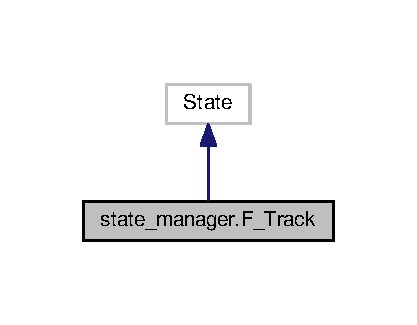
\includegraphics[width=200pt]{classstate__manager_1_1F__Track__inherit__graph}
\end{center}
\end{figure}


Collaboration diagram for state\+\_\+manager.\+F\+\_\+\+Track\+:\nopagebreak
\begin{figure}[H]
\begin{center}
\leavevmode
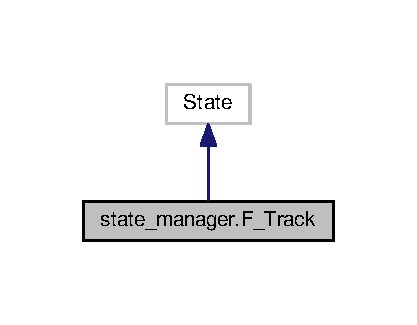
\includegraphics[width=200pt]{classstate__manager_1_1F__Track__coll__graph}
\end{center}
\end{figure}
\subsection*{Public Member Functions}
\begin{DoxyCompactItemize}
\item 
def \hyperlink{classstate__manager_1_1F__Track_ac6f957f5489c5115b2ba081448e48d35}{\+\_\+\+\_\+init\+\_\+\+\_\+} (self)
\begin{DoxyCompactList}\small\item\em Init function for smach machine normal state. \end{DoxyCompactList}\item 
def \hyperlink{classstate__manager_1_1F__Track_a95092e7c2a18a5eb83078ee9ccdfc07e}{execute} (self, userdata)
\begin{DoxyCompactList}\small\item\em Execute function of the state\+: \end{DoxyCompactList}\end{DoxyCompactItemize}


\subsection{Detailed Description}
Find track state of the smach machine. 



Definition at line 467 of file state\+\_\+manager.\+py.



\subsection{Constructor \& Destructor Documentation}
\index{state\+\_\+manager\+::\+F\+\_\+\+Track@{state\+\_\+manager\+::\+F\+\_\+\+Track}!\+\_\+\+\_\+init\+\_\+\+\_\+@{\+\_\+\+\_\+init\+\_\+\+\_\+}}
\index{\+\_\+\+\_\+init\+\_\+\+\_\+@{\+\_\+\+\_\+init\+\_\+\+\_\+}!state\+\_\+manager\+::\+F\+\_\+\+Track@{state\+\_\+manager\+::\+F\+\_\+\+Track}}
\subsubsection[{\texorpdfstring{\+\_\+\+\_\+init\+\_\+\+\_\+(self)}{__init__(self)}}]{\setlength{\rightskip}{0pt plus 5cm}def state\+\_\+manager.\+F\+\_\+\+Track.\+\_\+\+\_\+init\+\_\+\+\_\+ (
\begin{DoxyParamCaption}
\item[{}]{self}
\end{DoxyParamCaption}
)}\hypertarget{classstate__manager_1_1F__Track_ac6f957f5489c5115b2ba081448e48d35}{}\label{classstate__manager_1_1F__Track_ac6f957f5489c5115b2ba081448e48d35}


Init function for smach machine normal state. 



Definition at line 470 of file state\+\_\+manager.\+py.


\begin{DoxyCode}
470     \textcolor{keyword}{def }\hyperlink{classstate__manager_1_1F__Track_ac6f957f5489c5115b2ba081448e48d35}{\_\_init\_\_}(self):
471 
472         smach.State.\_\_init\_\_(self,
473                              outcomes=[\textcolor{stringliteral}{'find\_command'}, \textcolor{stringliteral}{'play\_command'}])
474 
\end{DoxyCode}


\subsection{Member Function Documentation}
\index{state\+\_\+manager\+::\+F\+\_\+\+Track@{state\+\_\+manager\+::\+F\+\_\+\+Track}!execute@{execute}}
\index{execute@{execute}!state\+\_\+manager\+::\+F\+\_\+\+Track@{state\+\_\+manager\+::\+F\+\_\+\+Track}}
\subsubsection[{\texorpdfstring{execute(self, userdata)}{execute(self, userdata)}}]{\setlength{\rightskip}{0pt plus 5cm}def state\+\_\+manager.\+F\+\_\+\+Track.\+execute (
\begin{DoxyParamCaption}
\item[{}]{self, }
\item[{}]{userdata}
\end{DoxyParamCaption}
)}\hypertarget{classstate__manager_1_1F__Track_a95092e7c2a18a5eb83078ee9ccdfc07e}{}\label{classstate__manager_1_1F__Track_a95092e7c2a18a5eb83078ee9ccdfc07e}


Execute function of the state\+: 


\begin{DoxyItemize}
\item Go close to the ball\+: is it the desired position? (no need to check if saved\+: u enter here only if it\textquotesingle{}s not)
\begin{DoxyItemize}
\item Yes\+: exit P\+L\+AY
\item No\+: exit F\+I\+ND 
\end{DoxyItemize}
\end{DoxyItemize}

Definition at line 480 of file state\+\_\+manager.\+py.


\begin{DoxyCode}
480     \textcolor{keyword}{def }\hyperlink{classstate__manager_1_1F__Track_a95092e7c2a18a5eb83078ee9ccdfc07e}{execute}(self, userdata):
481         \textcolor{keyword}{global} moveTo, vel\_pub, closeBall, justDetected, position\_, ballsPos, desiredRoom
482 
483         rospy.logerr(\textcolor{stringliteral}{'f\_track'})
484 
485         \textcolor{comment}{# Move closer to the ball}
486         \textcolor{keywordflow}{while} closeBall == -1:
487             vel\_to\_ball.angular.z = -0.002*(circCenter-400)
488             vel\_to\_ball.linear.x = -0.01*(radius-100)
489             vel\_pub.publish(vel\_to\_ball)
490 
491         \textcolor{comment}{# Stop dog}
492         rospy.logerr(\textcolor{stringliteral}{'Stopping in front of ball'})
493         \textcolor{keywordflow}{for} i \textcolor{keywordflow}{in} range(0, 3):
494             vel\_to\_ball.linear.x = 0
495             vel\_pub.publish(vel\_to\_ball)
496 
497         \textcolor{comment}{# If the ball is the one the human asked for, go back to play...}
498         \textcolor{keywordflow}{if} colorName[justDetected] == colorName[desiredRoom]:
499             rospy.logerr(\textcolor{stringliteral}{'I found the right ball'})
500 
501             \textcolor{comment}{# If not saved yet, save ball's position}
502             \textcolor{keywordflow}{if} ballsPos[justDetected] == [0, 0]:
503                 ballsPos[justDetected] = [position\_.x, position\_.y]
504                 rospy.logerr(
505                     \textcolor{stringliteral}{'Saved position of the %s ball, will not forget it!'}, colors[justDetected])
506 
507             \textcolor{keywordflow}{return} \textcolor{stringliteral}{'play\_command'}
508 
509         \textcolor{comment}{# ... if it is not, save its position anyway}
510         \textcolor{keywordflow}{else}:
511             rospy.logerr(
512                 \textcolor{stringliteral}{'I found the wrong ball'})
513 
514             \textcolor{comment}{# If not saved yet, save ball's position}
515             \textcolor{keywordflow}{if} ballsPos[justDetected] == [0, 0]:
516                 ballsPos[justDetected] = [position\_.x, position\_.y]
517                 rospy.logerr(
518                     \textcolor{stringliteral}{'Saved position of the %s ball anyway, may turn out useful'}, colors[justDetected])
519 
520             \textcolor{keywordflow}{return} \textcolor{stringliteral}{'find\_command'}
521 
\end{DoxyCode}


The documentation for this class was generated from the following file\+:\begin{DoxyCompactItemize}
\item 
scripts/\hyperlink{state__manager_8py}{state\+\_\+manager.\+py}\end{DoxyCompactItemize}

\hypertarget{classstate__manager_1_1MIRO__Find}{}\section{state\+\_\+manager.\+M\+I\+R\+O\+\_\+\+Find Class Reference}
\label{classstate__manager_1_1MIRO__Find}\index{state\+\_\+manager.\+M\+I\+R\+O\+\_\+\+Find@{state\+\_\+manager.\+M\+I\+R\+O\+\_\+\+Find}}


Find state of the smach machine.  




Inheritance diagram for state\+\_\+manager.\+M\+I\+R\+O\+\_\+\+Find\+:\nopagebreak
\begin{figure}[H]
\begin{center}
\leavevmode
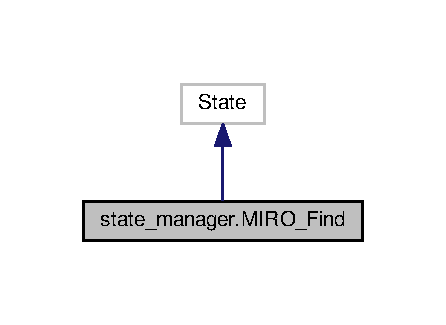
\includegraphics[width=214pt]{classstate__manager_1_1MIRO__Find__inherit__graph}
\end{center}
\end{figure}


Collaboration diagram for state\+\_\+manager.\+M\+I\+R\+O\+\_\+\+Find\+:\nopagebreak
\begin{figure}[H]
\begin{center}
\leavevmode
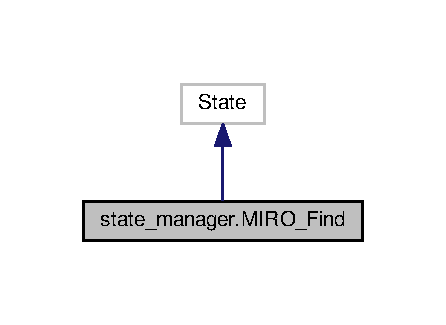
\includegraphics[width=214pt]{classstate__manager_1_1MIRO__Find__coll__graph}
\end{center}
\end{figure}
\subsection*{Public Member Functions}
\begin{DoxyCompactItemize}
\item 
def \hyperlink{classstate__manager_1_1MIRO__Find_a90643d8194779b79c594a23ad6e63e5a}{\+\_\+\+\_\+init\+\_\+\+\_\+} (self)
\begin{DoxyCompactList}\small\item\em Init function for smach machine normal state. \end{DoxyCompactList}\item 
def \hyperlink{classstate__manager_1_1MIRO__Find_a05ade27a9bfa1ad11e210be4373ff4a9}{execute} (self, userdata)
\begin{DoxyCompactList}\small\item\em Execute function of the state\+: \end{DoxyCompactList}\end{DoxyCompactItemize}


\subsection{Detailed Description}
Find state of the smach machine. 



Definition at line 421 of file state\+\_\+manager.\+py.



\subsection{Constructor \& Destructor Documentation}
\index{state\+\_\+manager\+::\+M\+I\+R\+O\+\_\+\+Find@{state\+\_\+manager\+::\+M\+I\+R\+O\+\_\+\+Find}!\+\_\+\+\_\+init\+\_\+\+\_\+@{\+\_\+\+\_\+init\+\_\+\+\_\+}}
\index{\+\_\+\+\_\+init\+\_\+\+\_\+@{\+\_\+\+\_\+init\+\_\+\+\_\+}!state\+\_\+manager\+::\+M\+I\+R\+O\+\_\+\+Find@{state\+\_\+manager\+::\+M\+I\+R\+O\+\_\+\+Find}}
\subsubsection[{\texorpdfstring{\+\_\+\+\_\+init\+\_\+\+\_\+(self)}{__init__(self)}}]{\setlength{\rightskip}{0pt plus 5cm}def state\+\_\+manager.\+M\+I\+R\+O\+\_\+\+Find.\+\_\+\+\_\+init\+\_\+\+\_\+ (
\begin{DoxyParamCaption}
\item[{}]{self}
\end{DoxyParamCaption}
)}\hypertarget{classstate__manager_1_1MIRO__Find_a90643d8194779b79c594a23ad6e63e5a}{}\label{classstate__manager_1_1MIRO__Find_a90643d8194779b79c594a23ad6e63e5a}


Init function for smach machine normal state. 



Definition at line 424 of file state\+\_\+manager.\+py.


\begin{DoxyCode}
424     \textcolor{keyword}{def }\hyperlink{classstate__manager_1_1MIRO__Find_a90643d8194779b79c594a23ad6e63e5a}{\_\_init\_\_}(self):
425 
426         smach.State.\_\_init\_\_(self,
427                              outcomes=[\textcolor{stringliteral}{'play\_command'}, \textcolor{stringliteral}{'f\_track\_command'}])
428 
\end{DoxyCode}


\subsection{Member Function Documentation}
\index{state\+\_\+manager\+::\+M\+I\+R\+O\+\_\+\+Find@{state\+\_\+manager\+::\+M\+I\+R\+O\+\_\+\+Find}!execute@{execute}}
\index{execute@{execute}!state\+\_\+manager\+::\+M\+I\+R\+O\+\_\+\+Find@{state\+\_\+manager\+::\+M\+I\+R\+O\+\_\+\+Find}}
\subsubsection[{\texorpdfstring{execute(self, userdata)}{execute(self, userdata)}}]{\setlength{\rightskip}{0pt plus 5cm}def state\+\_\+manager.\+M\+I\+R\+O\+\_\+\+Find.\+execute (
\begin{DoxyParamCaption}
\item[{}]{self, }
\item[{}]{userdata}
\end{DoxyParamCaption}
)}\hypertarget{classstate__manager_1_1MIRO__Find_a05ade27a9bfa1ad11e210be4373ff4a9}{}\label{classstate__manager_1_1MIRO__Find_a05ade27a9bfa1ad11e210be4373ff4a9}


Execute function of the state\+: 


\begin{DoxyItemize}
\item In a loop\+:
\item Move towards goal (may change it)\+: ball?
\begin{DoxyItemize}
\item Yes\+: exit F\+\_\+\+T\+R\+A\+CK
\item No\+: continue
\end{DoxyItemize}
\item End of the loop\+: exit P\+L\+AY 
\end{DoxyItemize}

Definition at line 436 of file state\+\_\+manager.\+py.


\begin{DoxyCode}
436     \textcolor{keyword}{def }\hyperlink{classstate__manager_1_1MIRO__Find_a05ade27a9bfa1ad11e210be4373ff4a9}{execute}(self, userdata):
437 
438         \textcolor{keyword}{global} justDetected
439 
440         rospy.logerr(\textcolor{stringliteral}{'find'})
441 
442         \textcolor{comment}{# Launch explore for autonomous exploration}
443         command2 = [\textcolor{stringliteral}{"roslaunch"}, \textcolor{stringliteral}{"explore\_lite"}, \textcolor{stringliteral}{"explore.launch"}]
444         p = subprocess.Popen(command2)
445 
446         \textcolor{keywordflow}{for} loops \textcolor{keywordflow}{in} range(0, 10):
447             time.sleep(1)
448 
449             \textcolor{keywordflow}{for} loops2 \textcolor{keywordflow}{in} range(0, LOOPS\_EXPLORE):
450                 time.sleep(3)
451 
452                 \textcolor{comment}{# Check if ball is detected}
453                 \textcolor{keywordflow}{if} justDetected != -1:
454                     rospy.logerr(\textcolor{stringliteral}{'I found something!'})
455                     p.terminate()
456                     time.sleep(7)
457 
458                     \textcolor{keywordflow}{return} \textcolor{stringliteral}{'f\_track\_command'}
459 
460         p.terminate()
461         time.sleep(7)
462 
463         \textcolor{keywordflow}{return} \textcolor{stringliteral}{'play\_command'}
464 
\end{DoxyCode}


The documentation for this class was generated from the following file\+:\begin{DoxyCompactItemize}
\item 
scripts/\hyperlink{state__manager_8py}{state\+\_\+manager.\+py}\end{DoxyCompactItemize}

\hypertarget{classstate__manager_1_1MIRO__Normal}{}\section{state\+\_\+manager.\+M\+I\+R\+O\+\_\+\+Normal Class Reference}
\label{classstate__manager_1_1MIRO__Normal}\index{state\+\_\+manager.\+M\+I\+R\+O\+\_\+\+Normal@{state\+\_\+manager.\+M\+I\+R\+O\+\_\+\+Normal}}


Normal state of the smach machine.  




Inheritance diagram for state\+\_\+manager.\+M\+I\+R\+O\+\_\+\+Normal\+:\nopagebreak
\begin{figure}[H]
\begin{center}
\leavevmode
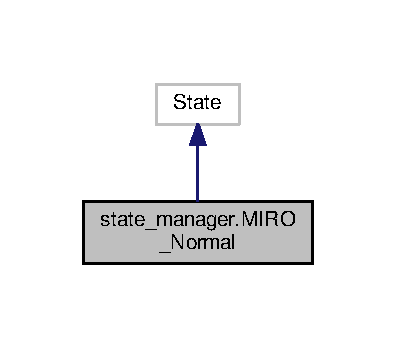
\includegraphics[width=190pt]{classstate__manager_1_1MIRO__Normal__inherit__graph}
\end{center}
\end{figure}


Collaboration diagram for state\+\_\+manager.\+M\+I\+R\+O\+\_\+\+Normal\+:\nopagebreak
\begin{figure}[H]
\begin{center}
\leavevmode
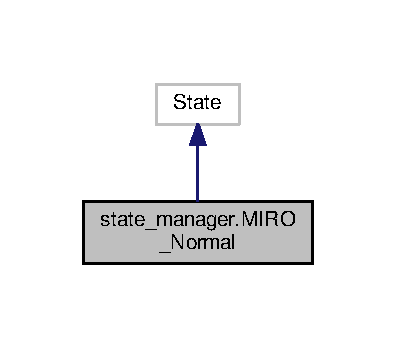
\includegraphics[width=190pt]{classstate__manager_1_1MIRO__Normal__coll__graph}
\end{center}
\end{figure}
\subsection*{Public Member Functions}
\begin{DoxyCompactItemize}
\item 
def \hyperlink{classstate__manager_1_1MIRO__Normal_a36a3ee79119b52beeebd6ee8c04d9501}{\+\_\+\+\_\+init\+\_\+\+\_\+} (self)
\begin{DoxyCompactList}\small\item\em Init function for smach machine normal state. \end{DoxyCompactList}\item 
def \hyperlink{classstate__manager_1_1MIRO__Normal_a4133da39ee6ec170623fc1d457b0729a}{execute} (self, userdata)
\begin{DoxyCompactList}\small\item\em Execute function of the state\+: \end{DoxyCompactList}\end{DoxyCompactItemize}


\subsection{Detailed Description}
Normal state of the smach machine. 



Definition at line 238 of file state\+\_\+manager.\+py.



\subsection{Constructor \& Destructor Documentation}
\index{state\+\_\+manager\+::\+M\+I\+R\+O\+\_\+\+Normal@{state\+\_\+manager\+::\+M\+I\+R\+O\+\_\+\+Normal}!\+\_\+\+\_\+init\+\_\+\+\_\+@{\+\_\+\+\_\+init\+\_\+\+\_\+}}
\index{\+\_\+\+\_\+init\+\_\+\+\_\+@{\+\_\+\+\_\+init\+\_\+\+\_\+}!state\+\_\+manager\+::\+M\+I\+R\+O\+\_\+\+Normal@{state\+\_\+manager\+::\+M\+I\+R\+O\+\_\+\+Normal}}
\subsubsection[{\texorpdfstring{\+\_\+\+\_\+init\+\_\+\+\_\+(self)}{__init__(self)}}]{\setlength{\rightskip}{0pt plus 5cm}def state\+\_\+manager.\+M\+I\+R\+O\+\_\+\+Normal.\+\_\+\+\_\+init\+\_\+\+\_\+ (
\begin{DoxyParamCaption}
\item[{}]{self}
\end{DoxyParamCaption}
)}\hypertarget{classstate__manager_1_1MIRO__Normal_a36a3ee79119b52beeebd6ee8c04d9501}{}\label{classstate__manager_1_1MIRO__Normal_a36a3ee79119b52beeebd6ee8c04d9501}


Init function for smach machine normal state. 



Definition at line 241 of file state\+\_\+manager.\+py.


\begin{DoxyCode}
241     \textcolor{keyword}{def }\hyperlink{classstate__manager_1_1MIRO__Normal_a36a3ee79119b52beeebd6ee8c04d9501}{\_\_init\_\_}(self):
242 
243         smach.State.\_\_init\_\_(self,
244                              outcomes=[\textcolor{stringliteral}{'sleep\_command'}, \textcolor{stringliteral}{'play\_command'}, \textcolor{stringliteral}{'n\_track\_command'}])
245 
\end{DoxyCode}


\subsection{Member Function Documentation}
\index{state\+\_\+manager\+::\+M\+I\+R\+O\+\_\+\+Normal@{state\+\_\+manager\+::\+M\+I\+R\+O\+\_\+\+Normal}!execute@{execute}}
\index{execute@{execute}!state\+\_\+manager\+::\+M\+I\+R\+O\+\_\+\+Normal@{state\+\_\+manager\+::\+M\+I\+R\+O\+\_\+\+Normal}}
\subsubsection[{\texorpdfstring{execute(self, userdata)}{execute(self, userdata)}}]{\setlength{\rightskip}{0pt plus 5cm}def state\+\_\+manager.\+M\+I\+R\+O\+\_\+\+Normal.\+execute (
\begin{DoxyParamCaption}
\item[{}]{self, }
\item[{}]{userdata}
\end{DoxyParamCaption}
)}\hypertarget{classstate__manager_1_1MIRO__Normal_a4133da39ee6ec170623fc1d457b0729a}{}\label{classstate__manager_1_1MIRO__Normal_a4133da39ee6ec170623fc1d457b0729a}


Execute function of the state\+: 


\begin{DoxyItemize}
\item Move around\+: ball?
\begin{DoxyItemize}
\item Yes\+: exit N\+\_\+\+T\+R\+A\+CK
\item No\+: Continue
\end{DoxyItemize}
\item Listen to human\+: play command?
\begin{DoxyItemize}
\item Yes\+: exit P\+L\+AY
\item No\+: Continue
\end{DoxyItemize}
\item End of the loop\+: exit S\+L\+E\+EP 
\end{DoxyItemize}

Definition at line 255 of file state\+\_\+manager.\+py.


\begin{DoxyCode}
255     \textcolor{keyword}{def }\hyperlink{classstate__manager_1_1MIRO__Normal_a4133da39ee6ec170623fc1d457b0729a}{execute}(self, userdata):
256         \textcolor{keyword}{global} justDetected, lastDetected
257 
258         rospy.logerr(\textcolor{stringliteral}{'normal'})
259         time.sleep(2)
260 
261         \textcolor{comment}{# Launch explore for autonomous exploration}
262         command = [\textcolor{stringliteral}{"roslaunch"}, \textcolor{stringliteral}{"explore\_lite"}, \textcolor{stringliteral}{"explore.launch"}]
263         p = subprocess.Popen(command)
264 
265         \textcolor{keywordflow}{for} loops \textcolor{keywordflow}{in} range(0, 10):
266             time.sleep(1)
267 
268             \textcolor{keywordflow}{for} loops2 \textcolor{keywordflow}{in} range(0, LOOPS\_EXPLORE):
269                 time.sleep(3)
270 
271                 \textcolor{comment}{# Check if ball is detected}
272                 \textcolor{keywordflow}{if} justDetected != -1:
273                     rospy.logerr(\textcolor{stringliteral}{'a ball was detected'})
274 
275                     \textcolor{comment}{# Check if it's a new ball or the same as before}
276                     \textcolor{keywordflow}{if} justDetected != lastDetected:
277                         lastDetected = justDetected
278                         rospy.logerr(\textcolor{stringliteral}{'and it is %s'}, colors[justDetected])
279 
280                         \textcolor{comment}{# Go to track state}
281                         p.terminate()
282                         time.sleep(7)
283 
284                         \textcolor{keywordflow}{return} \textcolor{stringliteral}{'n\_track\_command'}
285 
286                     \textcolor{keywordflow}{else}:
287                         rospy.logerr(\textcolor{stringliteral}{'but i already knew it'})
288 
289             \textcolor{comment}{# Listen to user}
290             \textcolor{keywordflow}{if} user\_says(0) == \textcolor{stringliteral}{'play'}:
291                 rospy.logerr(\textcolor{stringliteral}{'user said play'})
292 
293                 p.terminate()
294                 time.sleep(7)
295                 \textcolor{keywordflow}{return} \textcolor{stringliteral}{'play\_command'}
296 
297         p.terminate()
298         time.sleep(7)
299         \textcolor{keywordflow}{return} \textcolor{stringliteral}{'sleep\_command'}
300 
\end{DoxyCode}


The documentation for this class was generated from the following file\+:\begin{DoxyCompactItemize}
\item 
scripts/\hyperlink{state__manager_8py}{state\+\_\+manager.\+py}\end{DoxyCompactItemize}

\hypertarget{classstate__manager_1_1MIRO__Play}{}\section{state\+\_\+manager.\+M\+I\+R\+O\+\_\+\+Play Class Reference}
\label{classstate__manager_1_1MIRO__Play}\index{state\+\_\+manager.\+M\+I\+R\+O\+\_\+\+Play@{state\+\_\+manager.\+M\+I\+R\+O\+\_\+\+Play}}


Play state of the smach machine.  




Inheritance diagram for state\+\_\+manager.\+M\+I\+R\+O\+\_\+\+Play\+:\nopagebreak
\begin{figure}[H]
\begin{center}
\leavevmode
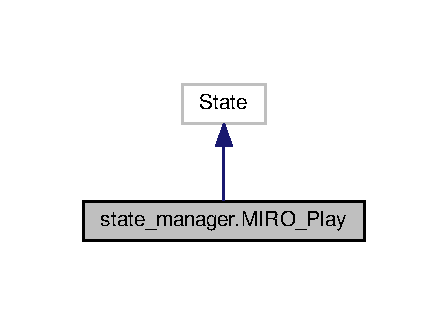
\includegraphics[width=215pt]{classstate__manager_1_1MIRO__Play__inherit__graph}
\end{center}
\end{figure}


Collaboration diagram for state\+\_\+manager.\+M\+I\+R\+O\+\_\+\+Play\+:\nopagebreak
\begin{figure}[H]
\begin{center}
\leavevmode
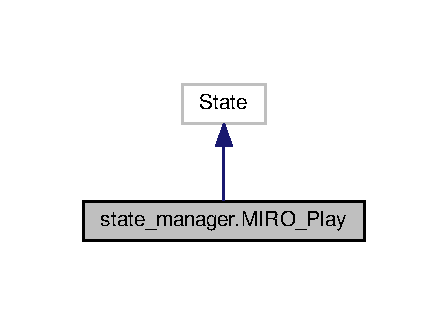
\includegraphics[width=215pt]{classstate__manager_1_1MIRO__Play__coll__graph}
\end{center}
\end{figure}
\subsection*{Public Member Functions}
\begin{DoxyCompactItemize}
\item 
def \hyperlink{classstate__manager_1_1MIRO__Play_a863ae1958460cf6bf33faaba597fc5a2}{\+\_\+\+\_\+init\+\_\+\+\_\+} (self)
\begin{DoxyCompactList}\small\item\em Init function for smach machine play state. \end{DoxyCompactList}\item 
def \hyperlink{classstate__manager_1_1MIRO__Play_a781db4be4fcbb313c46097a8fdf06275}{execute} (self, userdata)
\begin{DoxyCompactList}\small\item\em Execute function of the state\+: \end{DoxyCompactList}\end{DoxyCompactItemize}


\subsection{Detailed Description}
Play state of the smach machine. 



Definition at line 350 of file state\+\_\+manager.\+py.



\subsection{Constructor \& Destructor Documentation}
\index{state\+\_\+manager\+::\+M\+I\+R\+O\+\_\+\+Play@{state\+\_\+manager\+::\+M\+I\+R\+O\+\_\+\+Play}!\+\_\+\+\_\+init\+\_\+\+\_\+@{\+\_\+\+\_\+init\+\_\+\+\_\+}}
\index{\+\_\+\+\_\+init\+\_\+\+\_\+@{\+\_\+\+\_\+init\+\_\+\+\_\+}!state\+\_\+manager\+::\+M\+I\+R\+O\+\_\+\+Play@{state\+\_\+manager\+::\+M\+I\+R\+O\+\_\+\+Play}}
\subsubsection[{\texorpdfstring{\+\_\+\+\_\+init\+\_\+\+\_\+(self)}{__init__(self)}}]{\setlength{\rightskip}{0pt plus 5cm}def state\+\_\+manager.\+M\+I\+R\+O\+\_\+\+Play.\+\_\+\+\_\+init\+\_\+\+\_\+ (
\begin{DoxyParamCaption}
\item[{}]{self}
\end{DoxyParamCaption}
)}\hypertarget{classstate__manager_1_1MIRO__Play_a863ae1958460cf6bf33faaba597fc5a2}{}\label{classstate__manager_1_1MIRO__Play_a863ae1958460cf6bf33faaba597fc5a2}


Init function for smach machine play state. 



Definition at line 353 of file state\+\_\+manager.\+py.


\begin{DoxyCode}
353     \textcolor{keyword}{def }\hyperlink{classstate__manager_1_1MIRO__Play_a863ae1958460cf6bf33faaba597fc5a2}{\_\_init\_\_}(self):
354 
355         smach.State.\_\_init\_\_(self,
356                              outcomes=[\textcolor{stringliteral}{'normal\_command'}, \textcolor{stringliteral}{'find\_command'}])
357 
\end{DoxyCode}


\subsection{Member Function Documentation}
\index{state\+\_\+manager\+::\+M\+I\+R\+O\+\_\+\+Play@{state\+\_\+manager\+::\+M\+I\+R\+O\+\_\+\+Play}!execute@{execute}}
\index{execute@{execute}!state\+\_\+manager\+::\+M\+I\+R\+O\+\_\+\+Play@{state\+\_\+manager\+::\+M\+I\+R\+O\+\_\+\+Play}}
\subsubsection[{\texorpdfstring{execute(self, userdata)}{execute(self, userdata)}}]{\setlength{\rightskip}{0pt plus 5cm}def state\+\_\+manager.\+M\+I\+R\+O\+\_\+\+Play.\+execute (
\begin{DoxyParamCaption}
\item[{}]{self, }
\item[{}]{userdata}
\end{DoxyParamCaption}
)}\hypertarget{classstate__manager_1_1MIRO__Play_a781db4be4fcbb313c46097a8fdf06275}{}\label{classstate__manager_1_1MIRO__Play_a781db4be4fcbb313c46097a8fdf06275}


Execute function of the state\+: 


\begin{DoxyItemize}
\item In a loop\+:
\item Go to human
\item Wait for a goto command
\item Compare command to the known ball positions\+: is position known?
\begin{DoxyItemize}
\item Yes\+: go to position
\item No\+: exit F\+I\+ND
\end{DoxyItemize}
\item Wait to be arrived
\item End of the loop\+: exit N\+O\+R\+M\+AL 
\end{DoxyItemize}

Definition at line 368 of file state\+\_\+manager.\+py.


\begin{DoxyCode}
368     \textcolor{keyword}{def }\hyperlink{classstate__manager_1_1MIRO__Play_a781db4be4fcbb313c46097a8fdf06275}{execute}(self, userdata):
369         \textcolor{keyword}{global} moveTo, ballsPos, colorName, justDetected
370 
371         rospy.logerr(\textcolor{stringliteral}{'play'})
372         lastDetected = -2
373 
374         \textcolor{keywordflow}{if} ballsPos[0] != [0, 0] \textcolor{keywordflow}{and} ballsPos[1] != [0, 0] \textcolor{keywordflow}{and} ballsPos[2] != [0, 0] \textcolor{keywordflow}{and} ballsPos[3] != [0,
       0] \textcolor{keywordflow}{and} ballsPos[4] != [0, 0] \textcolor{keywordflow}{and} ballsPos[5] != [0, 0]:
375             rospy.logerr(\textcolor{stringliteral}{'ALL BALLS HAVE BEEN DETECTED! Positions:'})
376             rospy.logerr(ballsPos)
377 
378         \textcolor{keywordflow}{for} loops \textcolor{keywordflow}{in} range(0, 10):
379 
380             \textcolor{comment}{# Move to the human, unless dog is already near him}
381             rospy.logerr(\textcolor{stringliteral}{'moving to human'})
382             \textcolor{keywordflow}{if} (position\_.x > -7 \textcolor{keywordflow}{or} position\_.x < -3) \textcolor{keywordflow}{and} (position\_.y > 10 \textcolor{keywordflow}{or} position\_.y < 6):
383                 \textcolor{comment}{#move\_dog([-5, 8, 0])}
384                 time.sleep(1)
385 
386                 \textcolor{comment}{# Listen to human}
387             rospy.logerr(\textcolor{stringliteral}{'listen to user'})
388             user\_command = user\_says(1)
389 
390             \textcolor{comment}{# Save the desired room}
391             \textcolor{keywordflow}{if} \textcolor{stringliteral}{'go'} \textcolor{keywordflow}{in} user\_command \textcolor{keywordflow}{and} \textcolor{stringliteral}{'to'} \textcolor{keywordflow}{in} user\_command:
392                 \textcolor{keywordflow}{for} i \textcolor{keywordflow}{in} range(0, 6):
393                     \textcolor{keywordflow}{if} colorName[i] \textcolor{keywordflow}{in} user\_command:
394                         desiredRoom = i
395                         \textcolor{keywordflow}{break}
396 
397             \textcolor{keywordflow}{else}:
398                 rospy.logerr(\textcolor{stringliteral}{'Wrong command received'})
399                 \textcolor{keywordflow}{return} \textcolor{stringliteral}{'normal\_command'}
400 
401             rospy.logerr(\textcolor{stringliteral}{'user said to go to %s which is color %s'},
402                          colorName[desiredRoom], colors[desiredRoom])
403 
404             \textcolor{comment}{# If position of room (i.e. ball) is known, go there...}
405             \textcolor{keywordflow}{if} ballsPos[desiredRoom] != [0, 0]:
406                 rospy.logerr(
407                     \textcolor{stringliteral}{'i know this ball! i will go to it right away! it is in'})
408                 moveTo = np.append(np.asarray(ballsPos[desiredRoom]), 0)
409                 move\_dog(moveTo)
410 
411             \textcolor{comment}{# ... if not: look for it}
412             \textcolor{keywordflow}{else}:
413                 rospy.logerr(\textcolor{stringliteral}{'i do not know this position, i will look for it'})
414                 \textcolor{keywordflow}{return} \textcolor{stringliteral}{'find\_command'}
415 
416         \textcolor{keywordflow}{return} \textcolor{stringliteral}{'normal\_command'}
417 
418 
\end{DoxyCode}


The documentation for this class was generated from the following file\+:\begin{DoxyCompactItemize}
\item 
scripts/\hyperlink{state__manager_8py}{state\+\_\+manager.\+py}\end{DoxyCompactItemize}

\hypertarget{classstate__manager_1_1MIRO__Sleep}{}\section{state\+\_\+manager.\+M\+I\+R\+O\+\_\+\+Sleep Class Reference}
\label{classstate__manager_1_1MIRO__Sleep}\index{state\+\_\+manager.\+M\+I\+R\+O\+\_\+\+Sleep@{state\+\_\+manager.\+M\+I\+R\+O\+\_\+\+Sleep}}


Sleep state of the smach machine.  




Inheritance diagram for state\+\_\+manager.\+M\+I\+R\+O\+\_\+\+Sleep\+:\nopagebreak
\begin{figure}[H]
\begin{center}
\leavevmode
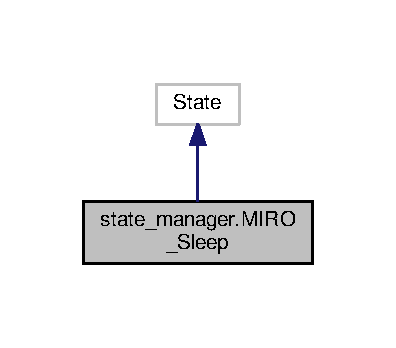
\includegraphics[width=190pt]{classstate__manager_1_1MIRO__Sleep__inherit__graph}
\end{center}
\end{figure}


Collaboration diagram for state\+\_\+manager.\+M\+I\+R\+O\+\_\+\+Sleep\+:\nopagebreak
\begin{figure}[H]
\begin{center}
\leavevmode
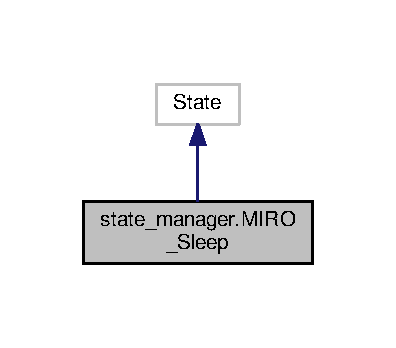
\includegraphics[width=190pt]{classstate__manager_1_1MIRO__Sleep__coll__graph}
\end{center}
\end{figure}
\subsection*{Public Member Functions}
\begin{DoxyCompactItemize}
\item 
def \hyperlink{classstate__manager_1_1MIRO__Sleep_a1e0695b96023b2c827bd28d9b0c11bfb}{\+\_\+\+\_\+init\+\_\+\+\_\+} (self)
\begin{DoxyCompactList}\small\item\em Init function for smach machine sleep state. \end{DoxyCompactList}\item 
def \hyperlink{classstate__manager_1_1MIRO__Sleep_acda704c667aad40c16f10d7c705b1b2e}{execute} (self, userdata)
\begin{DoxyCompactList}\small\item\em Execute function of the state\+: \end{DoxyCompactList}\end{DoxyCompactItemize}


\subsection{Detailed Description}
Sleep state of the smach machine. 



Definition at line 207 of file state\+\_\+manager.\+py.



\subsection{Constructor \& Destructor Documentation}
\index{state\+\_\+manager\+::\+M\+I\+R\+O\+\_\+\+Sleep@{state\+\_\+manager\+::\+M\+I\+R\+O\+\_\+\+Sleep}!\+\_\+\+\_\+init\+\_\+\+\_\+@{\+\_\+\+\_\+init\+\_\+\+\_\+}}
\index{\+\_\+\+\_\+init\+\_\+\+\_\+@{\+\_\+\+\_\+init\+\_\+\+\_\+}!state\+\_\+manager\+::\+M\+I\+R\+O\+\_\+\+Sleep@{state\+\_\+manager\+::\+M\+I\+R\+O\+\_\+\+Sleep}}
\subsubsection[{\texorpdfstring{\+\_\+\+\_\+init\+\_\+\+\_\+(self)}{__init__(self)}}]{\setlength{\rightskip}{0pt plus 5cm}def state\+\_\+manager.\+M\+I\+R\+O\+\_\+\+Sleep.\+\_\+\+\_\+init\+\_\+\+\_\+ (
\begin{DoxyParamCaption}
\item[{}]{self}
\end{DoxyParamCaption}
)}\hypertarget{classstate__manager_1_1MIRO__Sleep_a1e0695b96023b2c827bd28d9b0c11bfb}{}\label{classstate__manager_1_1MIRO__Sleep_a1e0695b96023b2c827bd28d9b0c11bfb}


Init function for smach machine sleep state. 



Definition at line 210 of file state\+\_\+manager.\+py.


\begin{DoxyCode}
210     \textcolor{keyword}{def }\hyperlink{classstate__manager_1_1MIRO__Sleep_a1e0695b96023b2c827bd28d9b0c11bfb}{\_\_init\_\_}(self):
211 
212         smach.State.\_\_init\_\_(self,
213                              outcomes=[\textcolor{stringliteral}{'normal\_command'}])
214 
\end{DoxyCode}


\subsection{Member Function Documentation}
\index{state\+\_\+manager\+::\+M\+I\+R\+O\+\_\+\+Sleep@{state\+\_\+manager\+::\+M\+I\+R\+O\+\_\+\+Sleep}!execute@{execute}}
\index{execute@{execute}!state\+\_\+manager\+::\+M\+I\+R\+O\+\_\+\+Sleep@{state\+\_\+manager\+::\+M\+I\+R\+O\+\_\+\+Sleep}}
\subsubsection[{\texorpdfstring{execute(self, userdata)}{execute(self, userdata)}}]{\setlength{\rightskip}{0pt plus 5cm}def state\+\_\+manager.\+M\+I\+R\+O\+\_\+\+Sleep.\+execute (
\begin{DoxyParamCaption}
\item[{}]{self, }
\item[{}]{userdata}
\end{DoxyParamCaption}
)}\hypertarget{classstate__manager_1_1MIRO__Sleep_acda704c667aad40c16f10d7c705b1b2e}{}\label{classstate__manager_1_1MIRO__Sleep_acda704c667aad40c16f10d7c705b1b2e}


Execute function of the state\+: 


\begin{DoxyItemize}
\item Go to kennel
\item Stay still for 5 seconds
\item Exit N\+O\+R\+M\+AL 
\end{DoxyItemize}

Definition at line 220 of file state\+\_\+manager.\+py.


\begin{DoxyCode}
220     \textcolor{keyword}{def }\hyperlink{classstate__manager_1_1MIRO__Sleep_acda704c667aad40c16f10d7c705b1b2e}{execute}(self, userdata):
221         \textcolor{keyword}{global} lastDetected
222         rospy.logerr(\textcolor{stringliteral}{'sleep'})
223 
224         \textcolor{comment}{# Go to kennel}
225         move\_dog([-5, 6, 0])
226         time.sleep(1)
227 
228         \textcolor{comment}{# Reset previously seen ball variable}
229         lastDetected = -2
230 
231         rospy.logerr(\textcolor{stringliteral}{'exit sleep'})
232         \textcolor{keywordflow}{return} \textcolor{stringliteral}{'normal\_command'}
233 
234 
\end{DoxyCode}


The documentation for this class was generated from the following file\+:\begin{DoxyCompactItemize}
\item 
scripts/\hyperlink{state__manager_8py}{state\+\_\+manager.\+py}\end{DoxyCompactItemize}

\hypertarget{classstate__manager_1_1N__Track}{}\section{state\+\_\+manager.\+N\+\_\+\+Track Class Reference}
\label{classstate__manager_1_1N__Track}\index{state\+\_\+manager.\+N\+\_\+\+Track@{state\+\_\+manager.\+N\+\_\+\+Track}}


Normal track state of the smach machine.  




Inheritance diagram for state\+\_\+manager.\+N\+\_\+\+Track\+:\nopagebreak
\begin{figure}[H]
\begin{center}
\leavevmode
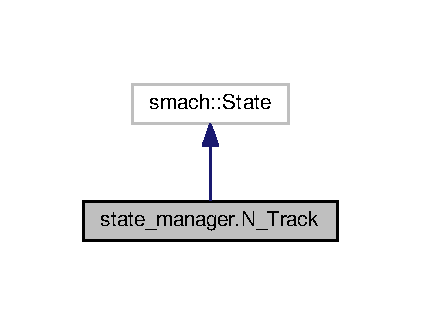
\includegraphics[width=202pt]{classstate__manager_1_1N__Track__inherit__graph}
\end{center}
\end{figure}


Collaboration diagram for state\+\_\+manager.\+N\+\_\+\+Track\+:\nopagebreak
\begin{figure}[H]
\begin{center}
\leavevmode
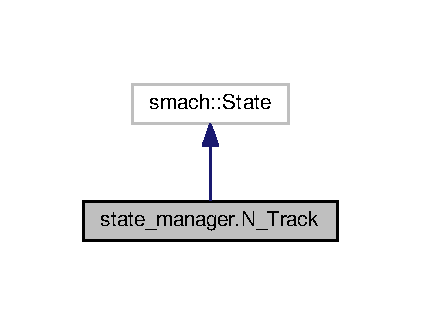
\includegraphics[width=202pt]{classstate__manager_1_1N__Track__coll__graph}
\end{center}
\end{figure}
\subsection*{Public Member Functions}
\begin{DoxyCompactItemize}
\item 
def \hyperlink{classstate__manager_1_1N__Track_aacd27d87838bc14f44bce9006219afe2}{\+\_\+\+\_\+init\+\_\+\+\_\+} (self)
\begin{DoxyCompactList}\small\item\em Init function for smach machine normal state. \end{DoxyCompactList}\item 
def \hyperlink{classstate__manager_1_1N__Track_ab05a0c6c37abff9d37e7e233553289d4}{execute} (self, userdata)
\begin{DoxyCompactList}\small\item\em Execute function of the state\+: \end{DoxyCompactList}\end{DoxyCompactItemize}


\subsection{Detailed Description}
Normal track state of the smach machine. 



Definition at line 303 of file state\+\_\+manager.\+py.



\subsection{Constructor \& Destructor Documentation}
\index{state\+\_\+manager\+::\+N\+\_\+\+Track@{state\+\_\+manager\+::\+N\+\_\+\+Track}!\+\_\+\+\_\+init\+\_\+\+\_\+@{\+\_\+\+\_\+init\+\_\+\+\_\+}}
\index{\+\_\+\+\_\+init\+\_\+\+\_\+@{\+\_\+\+\_\+init\+\_\+\+\_\+}!state\+\_\+manager\+::\+N\+\_\+\+Track@{state\+\_\+manager\+::\+N\+\_\+\+Track}}
\subsubsection[{\texorpdfstring{\+\_\+\+\_\+init\+\_\+\+\_\+(self)}{__init__(self)}}]{\setlength{\rightskip}{0pt plus 5cm}def state\+\_\+manager.\+N\+\_\+\+Track.\+\_\+\+\_\+init\+\_\+\+\_\+ (
\begin{DoxyParamCaption}
\item[{}]{self}
\end{DoxyParamCaption}
)}\hypertarget{classstate__manager_1_1N__Track_aacd27d87838bc14f44bce9006219afe2}{}\label{classstate__manager_1_1N__Track_aacd27d87838bc14f44bce9006219afe2}


Init function for smach machine normal state. 



Definition at line 306 of file state\+\_\+manager.\+py.


\begin{DoxyCode}
306     \textcolor{keyword}{def }\hyperlink{classstate__manager_1_1N__Track_aacd27d87838bc14f44bce9006219afe2}{\_\_init\_\_}(self):
307 
308         smach.State.\_\_init\_\_(self,
309                              outcomes=[\textcolor{stringliteral}{'normal\_command'}])
310 
\end{DoxyCode}


\subsection{Member Function Documentation}
\index{state\+\_\+manager\+::\+N\+\_\+\+Track@{state\+\_\+manager\+::\+N\+\_\+\+Track}!execute@{execute}}
\index{execute@{execute}!state\+\_\+manager\+::\+N\+\_\+\+Track@{state\+\_\+manager\+::\+N\+\_\+\+Track}}
\subsubsection[{\texorpdfstring{execute(self, userdata)}{execute(self, userdata)}}]{\setlength{\rightskip}{0pt plus 5cm}def state\+\_\+manager.\+N\+\_\+\+Track.\+execute (
\begin{DoxyParamCaption}
\item[{}]{self, }
\item[{}]{userdata}
\end{DoxyParamCaption}
)}\hypertarget{classstate__manager_1_1N__Track_ab05a0c6c37abff9d37e7e233553289d4}{}\label{classstate__manager_1_1N__Track_ab05a0c6c37abff9d37e7e233553289d4}


Execute function of the state\+: 


\begin{DoxyItemize}
\item Go close to the ball\+: did you know its position yet?
\begin{DoxyItemize}
\item Yes\+: continue
\item No\+: save it
\end{DoxyItemize}
\item Exit N\+O\+R\+M\+AL 
\end{DoxyItemize}

Definition at line 317 of file state\+\_\+manager.\+py.


\begin{DoxyCode}
317     \textcolor{keyword}{def }\hyperlink{classstate__manager_1_1N__Track_ab05a0c6c37abff9d37e7e233553289d4}{execute}(self, userdata):
318         \textcolor{keyword}{global} vel\_pub, closeBall, colorName, circCenter
319 
320         rospy.logerr(\textcolor{stringliteral}{'N\_track'})
321         time.sleep(2)
322 
323         \textcolor{comment}{# Move closer to the ball}
324         rospy.logerr(\textcolor{stringliteral}{'Moving closer to ball'})
325         \textcolor{keywordflow}{while} closeBall == -1:
326             vel\_to\_ball.angular.z = -0.002*(circCenter-400)
327             vel\_to\_ball.linear.x = -0.01*(radius-100)
328             vel\_pub.publish(vel\_to\_ball)
329 
330         \textcolor{comment}{# Stop dog}
331         rospy.logerr(\textcolor{stringliteral}{'Stopping in front of ball'})
332         \textcolor{keywordflow}{for} i \textcolor{keywordflow}{in} range(0, 3):
333             vel\_to\_ball.linear.x = 0
334             vel\_pub.publish(vel\_to\_ball)
335         time.sleep(3)
336 
337         \textcolor{comment}{# If not saved yet, save ball's position}
338         \textcolor{keywordflow}{if} ballsPos[justDetected] == [0, 0]:
339             ballsPos[justDetected] = [position\_.x, position\_.y]
340 
341             rospy.logerr(\textcolor{stringliteral}{'Saved position of %s ball as %d, %d approximately'},
342                          colors[justDetected], position\_.x, position\_.y)
343 
344         \textcolor{keywordflow}{return} \textcolor{stringliteral}{'normal\_command'}
345 
346 
\end{DoxyCode}


The documentation for this class was generated from the following file\+:\begin{DoxyCompactItemize}
\item 
scripts/\hyperlink{state__manager_8py}{state\+\_\+manager.\+py}\end{DoxyCompactItemize}

\chapter{File Documentation}
\hypertarget{camera__manager_8py}{}\section{scripts/camera\+\_\+manager.py File Reference}
\label{camera__manager_8py}\index{scripts/camera\+\_\+manager.\+py@{scripts/camera\+\_\+manager.\+py}}


Manages the camera, then sends relevant information (related to the ball) of the environment.  


\subsection*{Classes}
\begin{DoxyCompactItemize}
\item 
class \hyperlink{classcamera__manager_1_1camera__manager__fnct}{camera\+\_\+manager.\+camera\+\_\+manager\+\_\+fnct}
\begin{DoxyCompactList}\small\item\em Class to manage the camera. \end{DoxyCompactList}\end{DoxyCompactItemize}
\subsection*{Functions}
\begin{DoxyCompactItemize}
\item 
def \hyperlink{camera__manager_8py_aa1e2e246e891fb1387211d1286ec3147}{camera\+\_\+manager.\+camera\+\_\+manager} ()
\begin{DoxyCompactList}\small\item\em Ros node that subscribes to the target\+\_\+pos and odom topic and publishes on the cmd\+\_\+vel topic. \end{DoxyCompactList}\end{DoxyCompactItemize}
\subsection*{Variables}
\begin{DoxyCompactItemize}
\item 
tuple {\bfseries camera\+\_\+manager.\+black\+Lower} = (0, 0, 0)\hypertarget{camera__manager_8py_a0711994d37d741740e3584241c3668b0}{}\label{camera__manager_8py_a0711994d37d741740e3584241c3668b0}

\item 
tuple {\bfseries camera\+\_\+manager.\+black\+Upper} = (5, 50, 50)\hypertarget{camera__manager_8py_a1e3530ade7ba83681448c0b30a743b2b}{}\label{camera__manager_8py_a1e3530ade7ba83681448c0b30a743b2b}

\item 
tuple {\bfseries camera\+\_\+manager.\+red\+Lower} = (0, 50, 50)\hypertarget{camera__manager_8py_aa06654b05b11a238dc625d5342096949}{}\label{camera__manager_8py_aa06654b05b11a238dc625d5342096949}

\item 
tuple {\bfseries camera\+\_\+manager.\+red\+Upper} = (5, 255, 255)\hypertarget{camera__manager_8py_a23693497d0a2a2c43455d11625e05edf}{}\label{camera__manager_8py_a23693497d0a2a2c43455d11625e05edf}

\item 
tuple {\bfseries camera\+\_\+manager.\+yellow\+Lower} = (25, 50, 50)\hypertarget{camera__manager_8py_aa50588fa98b68e706fab3fd6bcabda9f}{}\label{camera__manager_8py_aa50588fa98b68e706fab3fd6bcabda9f}

\item 
tuple {\bfseries camera\+\_\+manager.\+yellow\+Upper} = (35, 255, 255)\hypertarget{camera__manager_8py_a2a5e03921dd37a7ebe93f2dfd66c9a4c}{}\label{camera__manager_8py_a2a5e03921dd37a7ebe93f2dfd66c9a4c}

\item 
tuple {\bfseries camera\+\_\+manager.\+green\+Lower} = (50, 50, 50)\hypertarget{camera__manager_8py_a013a8cf831e916d1bc0a38a3b85c3df9}{}\label{camera__manager_8py_a013a8cf831e916d1bc0a38a3b85c3df9}

\item 
tuple {\bfseries camera\+\_\+manager.\+green\+Upper} = (70, 255, 255)\hypertarget{camera__manager_8py_a1b03dd9aed1e6963c1e09fa5d04ae09f}{}\label{camera__manager_8py_a1b03dd9aed1e6963c1e09fa5d04ae09f}

\item 
tuple {\bfseries camera\+\_\+manager.\+blue\+Lower} = (100, 50, 50)\hypertarget{camera__manager_8py_a372ba4cb2d5a6e611e06c29e26c05529}{}\label{camera__manager_8py_a372ba4cb2d5a6e611e06c29e26c05529}

\item 
tuple {\bfseries camera\+\_\+manager.\+blue\+Upper} = (130, 255, 255)\hypertarget{camera__manager_8py_acb38a9a9b61af59df7786d99c8029868}{}\label{camera__manager_8py_acb38a9a9b61af59df7786d99c8029868}

\item 
tuple {\bfseries camera\+\_\+manager.\+magenta\+Lower} = (125, 50, 50)\hypertarget{camera__manager_8py_a09093eb6c6a6edd5389722127dad5bce}{}\label{camera__manager_8py_a09093eb6c6a6edd5389722127dad5bce}

\item 
tuple {\bfseries camera\+\_\+manager.\+magenta\+Upper} = (150, 255, 255)\hypertarget{camera__manager_8py_ac952d24444e8a70cfe9d6d39f5e2b802}{}\label{camera__manager_8py_ac952d24444e8a70cfe9d6d39f5e2b802}

\item 
list {\bfseries camera\+\_\+manager.\+lower\+Values}
\item 
list {\bfseries camera\+\_\+manager.\+upper\+Values}
\item 
list {\bfseries camera\+\_\+manager.\+color\+Name}
\item 
list {\bfseries camera\+\_\+manager.\+colors} = \mbox{[}\textquotesingle{}black\textquotesingle{}, \textquotesingle{}red\textquotesingle{}, \textquotesingle{}yellow\textquotesingle{}, \textquotesingle{}green\textquotesingle{}, \textquotesingle{}blue\textquotesingle{}, \textquotesingle{}magenta\textquotesingle{}\mbox{]}\hypertarget{camera__manager_8py_a6ff4e2963fe3e28f0ff83535518c87a6}{}\label{camera__manager_8py_a6ff4e2963fe3e28f0ff83535518c87a6}

\item 
list {\bfseries camera\+\_\+manager.\+black\+Pos} = \mbox{[}0, 0\mbox{]}\hypertarget{camera__manager_8py_a64a5746fc964f88e8858870ec1e2215f}{}\label{camera__manager_8py_a64a5746fc964f88e8858870ec1e2215f}

\item 
list {\bfseries camera\+\_\+manager.\+red\+Pos} = \mbox{[}0, 0\mbox{]}\hypertarget{camera__manager_8py_a7b148081ab6ff29076c1b2eb678c4803}{}\label{camera__manager_8py_a7b148081ab6ff29076c1b2eb678c4803}

\item 
list {\bfseries camera\+\_\+manager.\+yellow\+Pos} = \mbox{[}0, 0\mbox{]}\hypertarget{camera__manager_8py_ae83c232f66bf1e42c588d56632950dae}{}\label{camera__manager_8py_ae83c232f66bf1e42c588d56632950dae}

\item 
list {\bfseries camera\+\_\+manager.\+green\+Pos} = \mbox{[}0, 0\mbox{]}\hypertarget{camera__manager_8py_a7d6252ac8eef03f8133d169d1d495771}{}\label{camera__manager_8py_a7d6252ac8eef03f8133d169d1d495771}

\item 
list {\bfseries camera\+\_\+manager.\+blue\+Pos} = \mbox{[}0, 0\mbox{]}\hypertarget{camera__manager_8py_a9f13d5ad183dc84d577b9ae592e4f625}{}\label{camera__manager_8py_a9f13d5ad183dc84d577b9ae592e4f625}

\item 
list {\bfseries camera\+\_\+manager.\+magenta\+Pos} = \mbox{[}0, 0\mbox{]}\hypertarget{camera__manager_8py_a76332337890801ccd0aee5f998fa5190}{}\label{camera__manager_8py_a76332337890801ccd0aee5f998fa5190}

\item 
list {\bfseries camera\+\_\+manager.\+balls\+Pos} = \mbox{[}black\+Pos, red\+Pos, yellow\+Pos, green\+Pos, blue\+Pos, magenta\+Pos\mbox{]}\hypertarget{camera__manager_8py_a30fe654210baef33e6a554251d5ba8a9}{}\label{camera__manager_8py_a30fe654210baef33e6a554251d5ba8a9}

\item 
int {\bfseries camera\+\_\+manager.\+just\+Detected} = -\/1\hypertarget{camera__manager_8py_a4d18310539e0afde4b35045460153093}{}\label{camera__manager_8py_a4d18310539e0afde4b35045460153093}

\item 
int {\bfseries camera\+\_\+manager.\+close\+Ball} = -\/1\hypertarget{camera__manager_8py_a305e9918109c7ca854bb60a25eb0c67a}{}\label{camera__manager_8py_a305e9918109c7ca854bb60a25eb0c67a}

\item 
int {\bfseries camera\+\_\+manager.\+desired\+Room} = -\/1\hypertarget{camera__manager_8py_ac65f9de7b53620567919e0c2ad2f6184}{}\label{camera__manager_8py_ac65f9de7b53620567919e0c2ad2f6184}

\item 
{\bfseries camera\+\_\+manager.\+position\+\_\+} = Point()\hypertarget{camera__manager_8py_aa4eafdf8c597d236e56d1e05ffc2072c}{}\label{camera__manager_8py_aa4eafdf8c597d236e56d1e05ffc2072c}

\item 
{\bfseries camera\+\_\+manager.\+pose\+\_\+} = Pose()\hypertarget{camera__manager_8py_ad0a0b7e9b9e5aaf6c6ff3a81915170cf}{}\label{camera__manager_8py_ad0a0b7e9b9e5aaf6c6ff3a81915170cf}

\item 
int {\bfseries camera\+\_\+manager.\+yaw\+\_\+} = 0\hypertarget{camera__manager_8py_aa234a614cf2b170d030015accafd778d}{}\label{camera__manager_8py_aa234a614cf2b170d030015accafd778d}

\item 
int {\bfseries camera\+\_\+manager.\+yaw\+\_\+precision\+\_\+2\+\_\+} = 1\hypertarget{camera__manager_8py_af1640e282cedebfd46101221ab8df0fc}{}\label{camera__manager_8py_af1640e282cedebfd46101221ab8df0fc}

\item 
list {\bfseries camera\+\_\+manager.\+move\+To} = \mbox{[}0, 0, 0\mbox{]}\hypertarget{camera__manager_8py_ae8c290fb735787f7292c182a51c72711}{}\label{camera__manager_8py_ae8c290fb735787f7292c182a51c72711}

\item 
int {\bfseries camera\+\_\+manager.\+radius} = 0\hypertarget{camera__manager_8py_a591903b036f2e5552f7e9ed5881ae68f}{}\label{camera__manager_8py_a591903b036f2e5552f7e9ed5881ae68f}

\item 
int {\bfseries camera\+\_\+manager.\+circ\+Center} = 0\hypertarget{camera__manager_8py_a5608a02fa1ea9415474342446ed6bd9c}{}\label{camera__manager_8py_a5608a02fa1ea9415474342446ed6bd9c}

\end{DoxyCompactItemize}


\subsection{Detailed Description}
Manages the camera, then sends relevant information (related to the ball) of the environment. 



\subsection{Function Documentation}
\index{camera\+\_\+manager.\+py@{camera\+\_\+manager.\+py}!camera\+\_\+manager@{camera\+\_\+manager}}
\index{camera\+\_\+manager@{camera\+\_\+manager}!camera\+\_\+manager.\+py@{camera\+\_\+manager.\+py}}
\subsubsection[{\texorpdfstring{camera\+\_\+manager()}{camera_manager()}}]{\setlength{\rightskip}{0pt plus 5cm}def camera\+\_\+manager.\+camera\+\_\+manager (
\begin{DoxyParamCaption}
{}
\end{DoxyParamCaption}
)}\hypertarget{camera__manager_8py_file_aa1e2e246e891fb1387211d1286ec3147}{}\label{camera__manager_8py_file_aa1e2e246e891fb1387211d1286ec3147}


Ros node that subscribes to the target\+\_\+pos and odom topic and publishes on the cmd\+\_\+vel topic. 



Definition at line 163 of file camera\+\_\+manager.\+py.


\begin{DoxyCode}
163 \textcolor{keyword}{def }\hyperlink{namespacecamera__manager}{camera\_manager}():
164 
165     rospy.init\_node(\textcolor{stringliteral}{'camera\_manager'}, anonymous=\textcolor{keyword}{True})
166 
167     camera\_manager\_fnct()
168 
169     rospy.spin()
170 
171     \textcolor{keywordflow}{pass}
172 
173 
\end{DoxyCode}


\subsection{Variable Documentation}
\index{camera\+\_\+manager.\+py@{camera\+\_\+manager.\+py}!color\+Name@{color\+Name}}
\index{color\+Name@{color\+Name}!camera\+\_\+manager.\+py@{camera\+\_\+manager.\+py}}
\subsubsection[{\texorpdfstring{color\+Name}{colorName}}]{\setlength{\rightskip}{0pt plus 5cm}list camera\+\_\+manager.\+color\+Name}\hypertarget{camera__manager_8py_file_a9ac90360489eb398cfbb16994955c0ea}{}\label{camera__manager_8py_file_a9ac90360489eb398cfbb16994955c0ea}
{\bfseries Initial value\+:}
\begin{DoxyCode}
1 = [\textcolor{stringliteral}{'entrance'}, \textcolor{stringliteral}{'closet'}, \textcolor{stringliteral}{'kitchen'},
2              \textcolor{stringliteral}{'livingRoom'}, \textcolor{stringliteral}{'bedroom'}, \textcolor{stringliteral}{'bathroom'}]
\end{DoxyCode}


Definition at line 52 of file camera\+\_\+manager.\+py.

\index{camera\+\_\+manager.\+py@{camera\+\_\+manager.\+py}!lower\+Values@{lower\+Values}}
\index{lower\+Values@{lower\+Values}!camera\+\_\+manager.\+py@{camera\+\_\+manager.\+py}}
\subsubsection[{\texorpdfstring{lower\+Values}{lowerValues}}]{\setlength{\rightskip}{0pt plus 5cm}list camera\+\_\+manager.\+lower\+Values}\hypertarget{camera__manager_8py_file_aa60b3d1ff5b7713c1cbd9c1d015d765f}{}\label{camera__manager_8py_file_aa60b3d1ff5b7713c1cbd9c1d015d765f}
{\bfseries Initial value\+:}
\begin{DoxyCode}
1 = [blackLower, redLower, yellowLower,
2                greenLower, blueLower, magentaLower]
\end{DoxyCode}


Definition at line 48 of file camera\+\_\+manager.\+py.

\index{camera\+\_\+manager.\+py@{camera\+\_\+manager.\+py}!upper\+Values@{upper\+Values}}
\index{upper\+Values@{upper\+Values}!camera\+\_\+manager.\+py@{camera\+\_\+manager.\+py}}
\subsubsection[{\texorpdfstring{upper\+Values}{upperValues}}]{\setlength{\rightskip}{0pt plus 5cm}list camera\+\_\+manager.\+upper\+Values}\hypertarget{camera__manager_8py_file_a494feef841b62689595aa0e7554aba83}{}\label{camera__manager_8py_file_a494feef841b62689595aa0e7554aba83}
{\bfseries Initial value\+:}
\begin{DoxyCode}
1 = [blackUpper, redUpper, yellowUpper,
2                greenUpper, blueUpper, magentaUpper]
\end{DoxyCode}


Definition at line 50 of file camera\+\_\+manager.\+py.


\hypertarget{state__manager_8py}{}\section{scripts/state\+\_\+manager.py File Reference}
\label{state__manager_8py}\index{scripts/state\+\_\+manager.\+py@{scripts/state\+\_\+manager.\+py}}


Manges the dog behaviour states and the human commands.  


\subsection*{Classes}
\begin{DoxyCompactItemize}
\item 
class \hyperlink{classstate__manager_1_1MIRO__Sleep}{state\+\_\+manager.\+M\+I\+R\+O\+\_\+\+Sleep}
\begin{DoxyCompactList}\small\item\em Sleep state of the smach machine. \end{DoxyCompactList}\item 
class \hyperlink{classstate__manager_1_1MIRO__Normal}{state\+\_\+manager.\+M\+I\+R\+O\+\_\+\+Normal}
\begin{DoxyCompactList}\small\item\em Normal state of the smach machine. \end{DoxyCompactList}\item 
class \hyperlink{classstate__manager_1_1N__Track}{state\+\_\+manager.\+N\+\_\+\+Track}
\begin{DoxyCompactList}\small\item\em Normal track state of the smach machine. \end{DoxyCompactList}\item 
class \hyperlink{classstate__manager_1_1MIRO__Play}{state\+\_\+manager.\+M\+I\+R\+O\+\_\+\+Play}
\begin{DoxyCompactList}\small\item\em Play state of the smach machine. \end{DoxyCompactList}\item 
class \hyperlink{classstate__manager_1_1MIRO__Find}{state\+\_\+manager.\+M\+I\+R\+O\+\_\+\+Find}
\begin{DoxyCompactList}\small\item\em Find state of the smach machine. \end{DoxyCompactList}\item 
class \hyperlink{classstate__manager_1_1F__Track}{state\+\_\+manager.\+F\+\_\+\+Track}
\begin{DoxyCompactList}\small\item\em Find track state of the smach machine. \end{DoxyCompactList}\end{DoxyCompactItemize}
\subsection*{Functions}
\begin{DoxyCompactItemize}
\item 
def \hyperlink{state__manager_8py_a10b92f213f5d87f512d59297dc16b310}{state\+\_\+manager.\+clbk\+\_\+cam} (msg)\hypertarget{state__manager_8py_a10b92f213f5d87f512d59297dc16b310}{}\label{state__manager_8py_a10b92f213f5d87f512d59297dc16b310}

\begin{DoxyCompactList}\small\item\em Callback function for the camera information. \end{DoxyCompactList}\item 
def \hyperlink{state__manager_8py_aa8789198308cdcb1c68982937dc0325f}{state\+\_\+manager.\+user\+\_\+says} (state\+Calling)\hypertarget{state__manager_8py_aa8789198308cdcb1c68982937dc0325f}{}\label{state__manager_8py_aa8789198308cdcb1c68982937dc0325f}

\begin{DoxyCompactList}\small\item\em Function to simulate the human speaking. \end{DoxyCompactList}\item 
def \hyperlink{state__manager_8py_ae191ff1e095a04454793707dc8fed298}{state\+\_\+manager.\+clbk\+\_\+odom} (msg)\hypertarget{state__manager_8py_ae191ff1e095a04454793707dc8fed298}{}\label{state__manager_8py_ae191ff1e095a04454793707dc8fed298}

\begin{DoxyCompactList}\small\item\em Callback function for the odometry of the robot. \end{DoxyCompactList}\item 
def \hyperlink{state__manager_8py_a2642cd588f90cc3c9853d57f04925118}{state\+\_\+manager.\+normalize\+\_\+angle} (angle)\hypertarget{state__manager_8py_a2642cd588f90cc3c9853d57f04925118}{}\label{state__manager_8py_a2642cd588f90cc3c9853d57f04925118}

\begin{DoxyCompactList}\small\item\em Function to normalize the yaw angle. \end{DoxyCompactList}\item 
def \hyperlink{state__manager_8py_ae0155422a2f60744ea3acf5181c7c75a}{state\+\_\+manager.\+move\+\_\+dog} (target)
\begin{DoxyCompactList}\small\item\em Function to move the dog to a target position. \end{DoxyCompactList}\item 
def \hyperlink{state__manager_8py_a8663809bc92b964a1202b8888447a326}{state\+\_\+manager.\+main} ()\hypertarget{state__manager_8py_a8663809bc92b964a1202b8888447a326}{}\label{state__manager_8py_a8663809bc92b964a1202b8888447a326}

\begin{DoxyCompactList}\small\item\em Ros node that subscribes to camera\+\_\+info and odometry. \end{DoxyCompactList}\end{DoxyCompactItemize}
\subsection*{Variables}
\begin{DoxyCompactItemize}
\item 
list {\bfseries state\+\_\+manager.\+color\+Name}
\item 
list {\bfseries state\+\_\+manager.\+colors} = \mbox{[}\textquotesingle{}black\textquotesingle{}, \textquotesingle{}red\textquotesingle{}, \textquotesingle{}yellow\textquotesingle{}, \textquotesingle{}green\textquotesingle{}, \textquotesingle{}blue\textquotesingle{}, \textquotesingle{}magenta\textquotesingle{}\mbox{]}\hypertarget{state__manager_8py_a922042e614c40bebe0f29f4377f01b42}{}\label{state__manager_8py_a922042e614c40bebe0f29f4377f01b42}

\item 
list {\bfseries state\+\_\+manager.\+black\+Pos} = \mbox{[}0, 0\mbox{]}\hypertarget{state__manager_8py_aa4d3938ac74c8f777a1d8eb656fe7bb0}{}\label{state__manager_8py_aa4d3938ac74c8f777a1d8eb656fe7bb0}

\item 
list {\bfseries state\+\_\+manager.\+red\+Pos} = \mbox{[}0, 0\mbox{]}\hypertarget{state__manager_8py_ae0d8da1e5a3eb50004cb82db23cfe8e8}{}\label{state__manager_8py_ae0d8da1e5a3eb50004cb82db23cfe8e8}

\item 
list {\bfseries state\+\_\+manager.\+yellow\+Pos} = \mbox{[}0, 0\mbox{]}\hypertarget{state__manager_8py_a0b4119ef62fc8992409a95acaa413133}{}\label{state__manager_8py_a0b4119ef62fc8992409a95acaa413133}

\item 
list {\bfseries state\+\_\+manager.\+green\+Pos} = \mbox{[}0, 0\mbox{]}\hypertarget{state__manager_8py_ac90c0e9d4c30036629ea626868596af4}{}\label{state__manager_8py_ac90c0e9d4c30036629ea626868596af4}

\item 
list {\bfseries state\+\_\+manager.\+blue\+Pos} = \mbox{[}0, 0\mbox{]}\hypertarget{state__manager_8py_afb13d54268c086336e256dfbaad0d1be}{}\label{state__manager_8py_afb13d54268c086336e256dfbaad0d1be}

\item 
list {\bfseries state\+\_\+manager.\+magenta\+Pos} = \mbox{[}0, 0\mbox{]}\hypertarget{state__manager_8py_a8d1f33ece2a36276622cb4f8b716ed1c}{}\label{state__manager_8py_a8d1f33ece2a36276622cb4f8b716ed1c}

\item 
list {\bfseries state\+\_\+manager.\+balls\+Pos} = \mbox{[}black\+Pos, red\+Pos, yellow\+Pos, green\+Pos, blue\+Pos, magenta\+Pos\mbox{]}\hypertarget{state__manager_8py_aaa8c763e4fcef5460ec62aafbc9ac1ac}{}\label{state__manager_8py_aaa8c763e4fcef5460ec62aafbc9ac1ac}

\item 
int {\bfseries state\+\_\+manager.\+just\+Detected} = -\/1\hypertarget{state__manager_8py_afe71213bef1457af133e995ae8e89cf7}{}\label{state__manager_8py_afe71213bef1457af133e995ae8e89cf7}

\item 
int {\bfseries state\+\_\+manager.\+close\+Ball} = -\/1\hypertarget{state__manager_8py_a265a4ceebb76d5ed8ab531b56a9840c8}{}\label{state__manager_8py_a265a4ceebb76d5ed8ab531b56a9840c8}

\item 
int {\bfseries state\+\_\+manager.\+desired\+Room} = -\/1\hypertarget{state__manager_8py_aa3dc2e46764eb3a8533ff084e960ca56}{}\label{state__manager_8py_aa3dc2e46764eb3a8533ff084e960ca56}

\item 
int {\bfseries state\+\_\+manager.\+last\+Detected} = -\/2\hypertarget{state__manager_8py_af0f8b36f6452126a13d82ab1d19ec3cc}{}\label{state__manager_8py_af0f8b36f6452126a13d82ab1d19ec3cc}

\item 
int {\bfseries state\+\_\+manager.\+L\+O\+O\+P\+S\+\_\+\+E\+X\+P\+L\+O\+RE} = 20\hypertarget{state__manager_8py_a57e2d135527d81f9829dc7bfdb190077}{}\label{state__manager_8py_a57e2d135527d81f9829dc7bfdb190077}

\item 
{\bfseries state\+\_\+manager.\+position\+\_\+} = Point()\hypertarget{state__manager_8py_ac76fcb179cfa6a83beadd27948a07c75}{}\label{state__manager_8py_ac76fcb179cfa6a83beadd27948a07c75}

\item 
{\bfseries state\+\_\+manager.\+pose\+\_\+} = Pose()\hypertarget{state__manager_8py_ae34942bd07e8be3516ecf8d2b684f86f}{}\label{state__manager_8py_ae34942bd07e8be3516ecf8d2b684f86f}

\item 
int {\bfseries state\+\_\+manager.\+yaw\+\_\+} = 0\hypertarget{state__manager_8py_a07c3190cd1bf464f1a95c195764ec658}{}\label{state__manager_8py_a07c3190cd1bf464f1a95c195764ec658}

\item 
float {\bfseries state\+\_\+manager.\+yaw\+\_\+precision\+\_\+2\+\_\+} = 0.\+5\hypertarget{state__manager_8py_a54d071d5ed8358ee53a70ba15ba59fa2}{}\label{state__manager_8py_a54d071d5ed8358ee53a70ba15ba59fa2}

\item 
list {\bfseries state\+\_\+manager.\+move\+To} = \mbox{[}0, 0, 0\mbox{]}\hypertarget{state__manager_8py_a715b8f8103bafc082f0e8547b2d010cc}{}\label{state__manager_8py_a715b8f8103bafc082f0e8547b2d010cc}

\item 
{\bfseries state\+\_\+manager.\+vel\+\_\+pub} = rospy.\+Publisher(\char`\"{}/cmd\+\_\+vel\char`\"{}, Twist, queue\+\_\+size=1)\hypertarget{state__manager_8py_affa389297adfafddfa44cde69dfd3c2d}{}\label{state__manager_8py_affa389297adfafddfa44cde69dfd3c2d}

\item 
{\bfseries state\+\_\+manager.\+vel\+\_\+to\+\_\+ball} = Twist()\hypertarget{state__manager_8py_a227a8082ac335bc8bcc65bbf9847f847}{}\label{state__manager_8py_a227a8082ac335bc8bcc65bbf9847f847}

\item 
{\bfseries state\+\_\+manager.\+x}\hypertarget{state__manager_8py_a73b67913ce33b2f8a7b6ab9fdc2b4ac3}{}\label{state__manager_8py_a73b67913ce33b2f8a7b6ab9fdc2b4ac3}

\item 
{\bfseries state\+\_\+manager.\+y}\hypertarget{state__manager_8py_a71dbeef873718c59636bb7c58e163b5c}{}\label{state__manager_8py_a71dbeef873718c59636bb7c58e163b5c}

\item 
{\bfseries state\+\_\+manager.\+z}\hypertarget{state__manager_8py_a25495477e014402a47b01810bbb54416}{}\label{state__manager_8py_a25495477e014402a47b01810bbb54416}

\item 
int {\bfseries state\+\_\+manager.\+radius} = 0\hypertarget{state__manager_8py_acb974cb10e7943ddeacebed01c883d15}{}\label{state__manager_8py_acb974cb10e7943ddeacebed01c883d15}

\item 
int {\bfseries state\+\_\+manager.\+circ\+Center} = 0\hypertarget{state__manager_8py_a7c25469ab39caa485f115b5ff810e971}{}\label{state__manager_8py_a7c25469ab39caa485f115b5ff810e971}

\end{DoxyCompactItemize}


\subsection{Detailed Description}
Manges the dog behaviour states and the human commands. 



\subsection{Function Documentation}
\index{state\+\_\+manager.\+py@{state\+\_\+manager.\+py}!move\+\_\+dog@{move\+\_\+dog}}
\index{move\+\_\+dog@{move\+\_\+dog}!state\+\_\+manager.\+py@{state\+\_\+manager.\+py}}
\subsubsection[{\texorpdfstring{move\+\_\+dog(target)}{move_dog(target)}}]{\setlength{\rightskip}{0pt plus 5cm}def state\+\_\+manager.\+move\+\_\+dog (
\begin{DoxyParamCaption}
\item[{}]{target}
\end{DoxyParamCaption}
)}\hypertarget{state__manager_8py_file_ae0155422a2f60744ea3acf5181c7c75a}{}\label{state__manager_8py_file_ae0155422a2f60744ea3acf5181c7c75a}


Function to move the dog to a target position. 

It first sets the right yaw angle by directly publishing on the /cmd\+\_\+vel topic then implements a client to the Move\+Base service to move the robot to the target position while avoiding obstacles. 

Definition at line 147 of file state\+\_\+manager.\+py.


\begin{DoxyCode}
147 \textcolor{keyword}{def }move\_dog(target):
148     \textcolor{keyword}{global} yaw\_, pub, yaw\_precision\_2\_, vel\_pub, position\_
149 
150     kp\_a = 3.0
151     ub\_a = 0.6
152     lb\_a = -0.5
153 
154     rospy.logerr(\textcolor{stringliteral}{'move dog started with data %d %d'}, target[0], target[1])
155 
156     \textcolor{comment}{# Adjust yaw angle}
157     \textcolor{keywordflow}{while} \textcolor{keyword}{True}:
158         desired\_yaw = math.atan2(
159             target[1] - position\_.y, target[0] - position\_.x)
160         err\_yaw = normalize\_angle(desired\_yaw - yaw\_)
161 
162         twist\_msg = Twist()
163 
164         \textcolor{keywordflow}{if} math.fabs(err\_yaw) > yaw\_precision\_2\_:
165             twist\_msg.angular.z = kp\_a*err\_yaw
166             \textcolor{keywordflow}{if} twist\_msg.angular.z > ub\_a:
167                 twist\_msg.angular.z = ub\_a
168             \textcolor{keywordflow}{elif} twist\_msg.angular.z < lb\_a:
169                 twist\_msg.angular.z = lb\_a
170 
171         \textcolor{comment}{# Publish velocity directly on cmd\_vel topic}
172         vel\_pub.publish(twist\_msg)
173 
174         \textcolor{keywordflow}{if} math.fabs(err\_yaw) <= yaw\_precision\_2\_:
175             \textcolor{keywordflow}{break}
176 
177     \textcolor{comment}{# Move to target position}
178     rospy.logerr(\textcolor{stringliteral}{'now set target'})
179 
180     \textcolor{comment}{# Call MoveBase service}
181     client = actionlib.SimpleActionClient(\textcolor{stringliteral}{'move\_base'}, MoveBaseAction)
182     client.cancel\_goal
183     client.wait\_for\_server()
184 
185     goal = MoveBaseGoal()
186     goal.target\_pose.header.frame\_id = \textcolor{stringliteral}{"map"}
187     goal.target\_pose.header.stamp = rospy.Time.now()
188     goal.target\_pose.pose.position.x = target[0]
189     goal.target\_pose.pose.position.y = target[1]
190     goal.target\_pose.pose.position.z = 0
191     goal.target\_pose.pose.orientation.x = 0
192     goal.target\_pose.pose.orientation.y = 0
193     goal.target\_pose.pose.orientation.z = 0
194     goal.target\_pose.pose.orientation.w = 1.0
195 
196     client.send\_goal(goal)
197 
198     \textcolor{keywordflow}{while} math.fabs(position\_.x - target[0]) > 0.3 \textcolor{keywordflow}{or} math.fabs(position\_.y - target[1]) > 0.3:
199         time.sleep(1)
200     rospy.logerr(\textcolor{stringliteral}{'arrived'})
201     client.cancel\_all\_goals()
202     \textcolor{keywordflow}{return} 1
203 
204 
\end{DoxyCode}


\subsection{Variable Documentation}
\index{state\+\_\+manager.\+py@{state\+\_\+manager.\+py}!color\+Name@{color\+Name}}
\index{color\+Name@{color\+Name}!state\+\_\+manager.\+py@{state\+\_\+manager.\+py}}
\subsubsection[{\texorpdfstring{color\+Name}{colorName}}]{\setlength{\rightskip}{0pt plus 5cm}list state\+\_\+manager.\+color\+Name}\hypertarget{state__manager_8py_file_a1a31c151159de59b0bd90954a51f4de0}{}\label{state__manager_8py_file_a1a31c151159de59b0bd90954a51f4de0}
{\bfseries Initial value\+:}
\begin{DoxyCode}
1 = [\textcolor{stringliteral}{'entrance'}, \textcolor{stringliteral}{'closet'}, \textcolor{stringliteral}{'kitchen'},
2              \textcolor{stringliteral}{'livingRoom'}, \textcolor{stringliteral}{'bedroom'}, \textcolor{stringliteral}{'bathroom'}]
\end{DoxyCode}


Definition at line 36 of file state\+\_\+manager.\+py.


%--- End generated contents ---

% Index
\backmatter
\newpage
\phantomsection
\clearemptydoublepage
\addcontentsline{toc}{chapter}{Index}
\printindex

\end{document}
